\documentclass[11pt]{article}
\usepackage[fontset=fandol]{ctex}
\usepackage{amsmath,amssymb}
\usepackage{array,booktabs}
\usepackage{graphicx,xcolor}
\usepackage[
    paperwidth=320mm,paperheight=180mm,
    left=17mm,right=17mm,top=12mm,bottom=15mm,footskip=9mm
]{geometry}
\usepackage{hyperref}

\definecolor{SlideHeading}{HTML}{152B42}
\definecolor{SlideText}{HTML}{203044}
\definecolor{SlideAccent}{HTML}{116968}
\hypersetup{
    pdftitle={Agent测试时计算扩展},
    pdfstartview=Fit,
    colorlinks=true,urlcolor=SlideAccent,linkcolor=SlideAccent
}

\makeatletter
\newcommand{\ps@slides}{%
    \let\@oddhead\@empty
    \let\@evenhead\@empty
    \def\@oddfoot{\hfil{\rmfamily\fontsize{13}{16}\selectfont\color{SlideAccent}\thepage}}%
    \let\@evenfoot\@oddfoot
}
\renewcommand{\@listi}{%
    \leftmargin\leftmargini
    \topsep6pt
    \itemsep7pt
    \parsep0pt
    \partopsep0pt
}
\let\@listI\@listi
\makeatother

\newcommand{\slidetitle}[2][1]{%
    \clearpage
    \pdfbookmark[#1]{#2}{slide.\thepage}%
    {\color{SlideHeading}\bfseries\fontsize{32}{40}\selectfont #2\par}%
    \vspace{3mm}%
}

\newcommand{\slideimage}[2][110mm]{%
    {\centering
    \includegraphics[width=\linewidth,height=#1,keepaspectratio]{figures/#2}\par}%
}

\begin{document}
\pagestyle{slides}
\raggedright
\rmfamily
\linespread{1}
\fontsize{20}{29}\selectfont
\color{SlideText}
\setlength{\parindent}{0pt}
\setlength{\parskip}{8pt}
\setlength{\leftmargini}{1.6em}
\renewcommand{\arraystretch}{1.4}

\thispagestyle{empty}
\pdfbookmark[0]{Agent测试时计算扩展}{cover}
\vspace*{18mm}
{\color{SlideHeading}\bfseries\fontsize{49}{59}\selectfont Agent测试时计算扩展\par}
\vspace{8mm}
{\color{SlideAccent}\bfseries\fontsize{24}{31}\selectfont 相关论文\par}
\begin{enumerate}
    \item Large Language Monkeys: Scaling Inference Compute with Repeated Sampling
    \item Scaling LLM Test-Time Compute Optimally can be More Effective \mbox{than Scaling Model Parameters}
    \item Archon: An Architecture Search Framework for Inference-Time Techniques
\end{enumerate}

\slidetitle[0]{固定模型下的推理计算}

训练阶段的 scaling law 描述训练计算量与模型性能的关系。

{\bfseries\fontsize{24}{34}\selectfont
在模型参数固定以后，能否通过更多采样、搜索、修订和验证，\\
提高同一个模型的最终成功率？\par}

\begin{enumerate}
    \item \textbf{Large Language Monkeys}\quad 重复采样为什么呈现可预测的 scaling law？
    \item \textbf{Compute-optimal test-time scaling}\quad 并行采样和串行修订应如何分配预算？
    \item \textbf{Archon}\quad 如何自动搜索由 generator、critic、ranker、fuser 和 verifier 组成的推理架构？
\end{enumerate}

\slidetitle{候选覆盖率与选择策略}

\textbf{生成}决定候选集能否覆盖正确解，\textbf{验证}决定能否识别正确解，\textbf{预算分配}决定有限计算能否用在收益最高的操作上。

\begin{tabular}{@{}p{.26\linewidth}p{.69\linewidth}@{}}
\toprule
\textbf{指标或策略} & \textbf{含义} \\
\midrule
pass@1 & 系统只交付一个答案时的最终准确率 \\
pass@$k$ / coverage & $k$ 个候选中至少存在一个正确答案的概率 \\
best-of-$N$ & 生成 $N$ 个候选后，由 verifier 选择一个答案 \\
majority@$N$ & 按答案频率投票，假设正确答案最常出现 \\
\bottomrule
\end{tabular}

系统最终只交付一个答案，因此需要分别测量 coverage 与 pass@1。比较策略时，还需要权衡候选质量、选择质量与计算成本。

\slidetitle[0]{Large Language Monkeys 的生成与验证流程}

\slideimage[102mm]{generate-verify.jpg}

Repeated sampling 从同一模型独立采样多个候选，再交给 verifier 选择。单元测试、编译器和 proof checker 可为代码与形式化证明提供自动反馈。

\slidetitle{单题 coverage 随采样次数饱和}

对问题 $i$ 独立采样 $k$ 次时，oracle coverage 等于至少一次采样成功的概率。

\[
C_i(k)=1-(1-p_i)^k.
\]

\begin{itemize}
    \item $p_i$\quad 模型对问题 $i$ 的单次成功概率。
    \item $k$\quad 采样数。
    \item $C_i(k)$\quad 候选集合至少包含一个正确解的概率。
\end{itemize}

当 $0<p_i<1$ 时，初始采样的边际收益最大，之后逐步下降。

\slidetitle{小模型为何能通过采样追上强模型}

\slideimage[98mm]{repeated-sampling.jpg}

大量采样缩小了小模型与强模型单次推理的差距。实验覆盖数学、代码与形式化证明。

\textbf{能力被“放大”还是被“发现”？}采样越多，越容易找到已有的低概率正确轨迹。

\slidetitle{数据集平均 coverage 的经验拟合}

平均 coverage 随采样数变化，可用 \mbox{exponentiated power law} 拟合。

\[
\begin{gathered}
\bar C(k)\approx 1-\exp(-a k^b),\\
a>0,\quad 0<b<1.
\end{gathered}
\]

\begin{itemize}
    \item $\bar C(k)$\quad 数据集上的平均 coverage。
    \item $a$\quad 与模型和任务总体难度相关的尺度参数。
    \item $b$\quad 控制 scaling 速度的指数。
    \item $k$\quad 推理采样预算。
\end{itemize}

\slidetitle{为什么对问题取平均后会出现幂律？}

单题 coverage 按 $1-(1-p_i)^k$ 指数饱和。许多模型偶尔才能解出的难题在 $p_i$ 接近零的位置形成长尾。

若单次成功概率在 $p\rightarrow0$ 附近具有密度
\[
f(p)\propto p^{\alpha-1},
\]
其中 $\alpha$ 是靠近零点的长尾指数，则数据集平均失败率近似为
\[
1-\bar C(k)=\mathbb{E}_{p}[(1-p)^k]
\approx\int_{0}^{\infty} e^{-kp}p^{\alpha-1}\,dp
\propto k^{-\alpha}.
\]

\slidetitle{长尾决定采样收益何时饱和}

\slideimage[99mm]{long-tail-theorem.jpg}

如果题目的 $p_i$ 普遍较高，少量采样后就会饱和。如果大量题目的 $p_i$ 极低但非零，收益会延续到很大的 $k$。推理 scaling 也取决于 benchmark 的难度分布。

\slidetitle{预训练与推理的预算权衡}

\slideimage[99mm]{compute-allocation.jpg}

如果基础模型偶尔能生成正确解，且 verifier 能识别这类候选，按请求增加推理计算就可能提高成功率。对少量高价值请求，这可能比训练和部署更大的模型更经济。

\slidetitle[0]{Generation-Verification Gap}

\textbf{Oracle coverage 是固定候选集下的准确率上界。}只要候选集中有正确答案，知道 ground truth 的 oracle verifier 就能选中它。

\[
G(k)=C_{\mathrm{oracle}}(k)-A_{\mathrm{selector}}(k).
\]

\begin{itemize}
    \item $C_{\mathrm{oracle}}(k)$\quad 候选集合中存在正确答案的比例。
    \item $A_{\mathrm{selector}}(k)$\quad 真实选择器交付正确答案的比例。
    \item $G(k)$\quad generation-verification gap。
\end{itemize}

\slidetitle{候选覆盖率与实际准确率的差距}

\slideimage[108mm]{verification-gap.jpg}

实际选择器通常使用多数投票、reward model 或 LLM judge，最终准确率可能远低于 oracle coverage。

\slidetitle{为什么 majority vote 会失败}

\slideimage[97mm]{rare-correct.jpg}

Self-consistency 依赖正确答案比任一错误答案更常出现。如果模型反复生成同一种错误，增加采样会让投票结果更稳定地偏向该错误。候选间的一致性反映答案出现的频率，正确性仍需验证。

\slidetitle{验证器应具备什么性质}

\begin{itemize}
    \item \textbf{Soundness}\quad 拒绝明显错误的候选。
    \item \textbf{Recall}\quad 尽可能识别候选中的稀有正确解。
    \item \textbf{Calibration}\quad 评分应反映实际成功概率。
    \item \textbf{Robustness}\quad 对候选的风格、长度和表面自信保持稳健。
    \item \textbf{Cost}\quad 验证成本应显著低于重新生成或人工检查。
\end{itemize}

形式化证明和代码执行可借助符号系统或真实环境。开放式任务更难低成本获取 ground truth，通常依赖 learned reward model 或延迟反馈。

生成器变强或采样增多时，候选分布可能更复杂，稀有正确解也可能更难识别。

\slidetitle[0]{Compute-Optimal Test-Time Scaling}

\begin{minipage}[c]{.41\linewidth}
\raggedright
\textbf{并行采样（Parallel sampling）}

从同一 prompt 独立生成多个候选，扩大搜索宽度。错误不会跨候选传播。

\medskip
\textbf{串行修订（Sequential revision）}

读取中间结果并逐步修订，增加单条轨迹的搜索深度。早期错误可能影响后续修订。
\end{minipage}\hfill
\begin{minipage}[c]{.57\linewidth}
    \slideimage{parallel-sampling.jpg}
\end{minipage}

\slidetitle{Outcome Reward Model 与 Process Reward Model}

\begin{minipage}[c]{.44\linewidth}
\raggedright
\setlength{\parskip}{8pt}
\textbf{ORM} 只评价最终答案，适合 best-of-$N$。信用分配较粗。

\textbf{PRM} 逐步评价推理过程，为 beam search 和提前剪枝提供信号。

对包含步骤 $z_{1:T}$ 的轨迹，PRM 给出局部得分
\[
r_t=r(z_t\mid z_{<t},x),
\]
帮助搜索器在生成完整答案前保留高潜力分支。
\end{minipage}\hfill
\begin{minipage}[c]{.54\linewidth}
    \slideimage{reward-model-types.jpg}
\end{minipage}

\slidetitle{组合搜索宽度与深度}

\slideimage[108mm]{hybrid-search.jpg}

系统可以先并行探索多个初始候选，再对高分候选进行多轮串行修订。

\slidetitle{单题总推理预算}

并行采样、串行修订与验证共用预算 $B$。

\[
B=n_{\mathrm{parallel}}\cdot c_{\mathrm{sample}}
+n_{\mathrm{revise}}\cdot c_{\mathrm{revise}}
+c_{\mathrm{verify}}.
\]

\begin{itemize}
    \item $n_{\mathrm{parallel}}$\quad 并行候选数。
    \item $n_{\mathrm{revise}}$\quad 串行修订轮数。
    \item $c_{\mathrm{sample}},c_{\mathrm{revise}},c_{\mathrm{verify}}$\quad 各操作成本。
\end{itemize}

\slidetitle{PRM 指导下的搜索收益}

\slideimage[109mm]{compute-optimal-results.jpg}

在 PRM 指导下，compute-optimal search 的早期收益高于纯 best-of-$N$。

\slidetitle{最优预算分配随问题难度变化}

\slideimage[100mm]{parallel-sequential-ratio.jpg}

简单题往往已有接近正确的初始解，串行修订可以快速纠正。困难题的初始解可能落入错误思路，需要并行探索不同方向。

\slidetitle{测试时 FLOPs 何时胜过预训练 FLOPs}

\slideimage[100mm]{testtime-vs-pretraining.jpg}

中等难度问题常从 test-time compute 获益。基础模型几乎采样不到正确轨迹时，增加搜索的收益有限，扩大预训练或改进训练数据更可能改善表现。

\slidetitle{在线预算分配}

\begin{itemize}
    \item 过度串行会把预算耗在修补方向错误的轨迹上。
    \item 过度并行会产生大量浅层候选，反馈利用不足。
\end{itemize}

在线调度根据问题难度、模型能力和 verifier 质量估计边际收益，据此选择继续采样、修订、验证或停止。

\slidetitle[0]{Archon 将推理系统视为可搜索架构}

\slideimage[98mm]{archon-framework.jpg}

给定目标任务、候选模型、可用操作和成本约束，Archon 借用神经网络的分层结构组织推理操作，搜索各层的操作组合、顺序、模型来源和调用次数，得到一张执行图。

\slidetitle{Archon 操作的输入、输出与成本}

% Remove the white margins of the original screenshot to enlarge the table.
{\centering
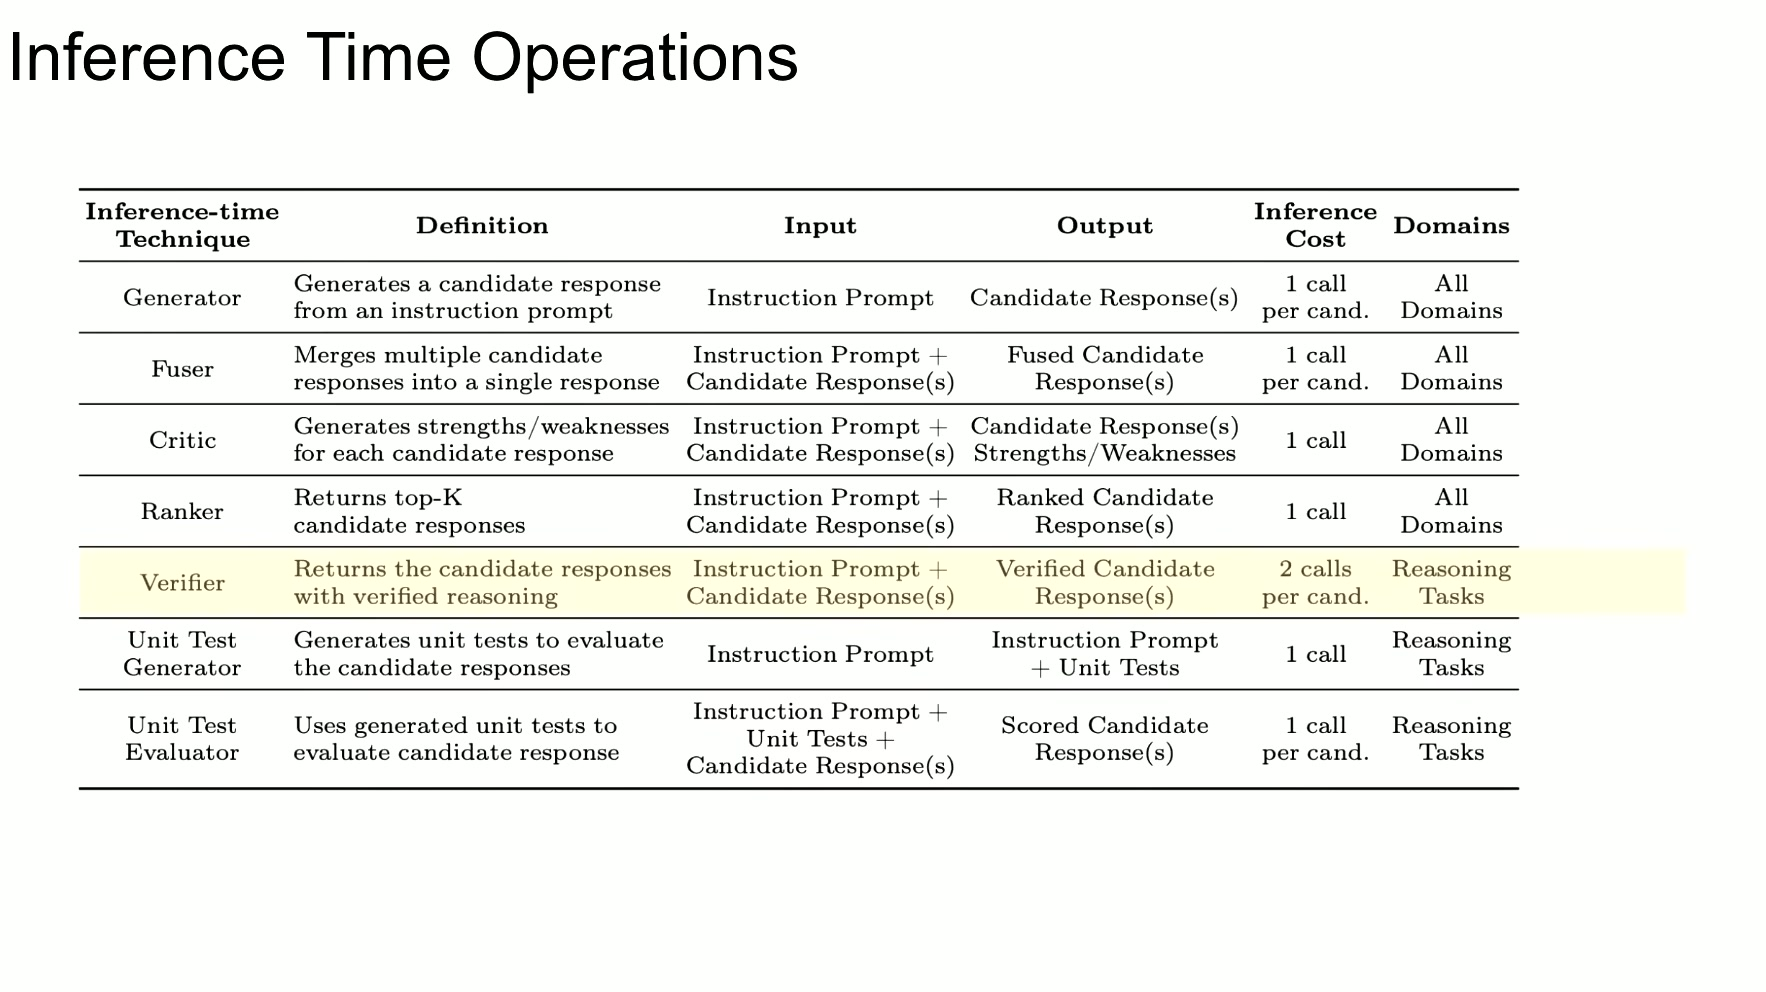
\includegraphics[
    width=\linewidth,height=124mm,keepaspectratio,
    trim=0bp 176bp 210bp 12bp,clip
]{figures/archon-operations.jpg}\par}

\slidetitle{可组合操作及主要风险}

\begin{tabular}{@{}p{.21\linewidth}p{.36\linewidth}p{.38\linewidth}@{}}
\toprule
\textbf{操作} & \textbf{功能} & \textbf{主要风险} \\
\midrule
Generator & 产生一个或多个候选 & 缺乏多样性、重复错误 \\
Critic & 指出候选缺陷与遗漏 & 批评不准确或只关注表面形式 \\
Ranker & 对候选排序 & 位置偏差、长度偏差、judge 偏差 \\
Fuser & 综合多个候选的互补部分 & 把错误也融合进去 \\
Verifier / Tests & 检查约束与正确性 & 测试覆盖不足、奖励投机 \\
\bottomrule
\end{tabular}

\slidetitle{Fusion 为什么可能超过 oracle selection}

\slideimage[98mm]{fusion-results.jpg}

Oracle selection 的上界适用于固定候选集。Fuser 可以通过额外的模型调用，把多个候选中的互补信息融合为新答案，从而改变候选空间。

\slidetitle{自然语言单元测试}

\slideimage[95mm]{natural-language-tests.jpg}

缺少可执行的 ground truth 时，Archon 让模型生成自然语言测试来检查候选。模型可能遗漏关键需求，因此可以结合用户要求和领域规则构建检查条件。

\slidetitle{多层推理架构}

\slideimage[101mm]{archon-architectures.jpg}

多个 generator 可以并行采样，由 critic 识别缺陷，ranker 选择候选，fuser 综合答案，再进行下一轮批评与融合。

\slidetitle{多层架构的贝叶斯搜索}

\slideimage[103mm]{bayesian-search.jpg}

层数、操作类型、模型和超参数共同扩大搜索空间。实验中，贝叶斯优化比随机或贪心搜索更高效地找到高性能配置。

\slidetitle{架构搜索的目标函数}

配置 $a$ 的综合效用同时衡量质量、成本与延迟。

\[
J(a)=\mathrm{Quality}(a)-\lambda_c\mathrm{Cost}(a)-\lambda_l\mathrm{Latency}(a).
\]

\begin{itemize}
    \item $\mathrm{Quality}(a)$\quad 目标 benchmark 上的准确率或偏好分。
    \item $\mathrm{Cost}(a)$\quad 模型调用和 token 成本。
    \item $\mathrm{Latency}(a)$\quad 关键路径延迟。
    \item $\lambda_c,\lambda_l$\quad 部署场景对成本与延迟的权重。
\end{itemize}

\slidetitle{Archon 在不同模型池上的实验结果}

\slideimage[118mm]{archon-results.jpg}

Archon 在开源、闭源与混合模型池上取得稳定提升。

\slidetitle{架构搜索的收益与代价}

Archon 把 prompt engineering 扩展为系统架构搜索，在成本约束下优化多个模型调用之间的数据流和控制流。

\begin{itemize}
    \item 搜索结果可能过拟合 benchmark。
    \item 更复杂的架构可能增加延迟和维护成本，降低系统的可解释性。
\end{itemize}

\slidetitle[0]{哪些任务适合增加推理预算？}

\begin{enumerate}
    \item 基础模型是否偶尔能产生正确答案，即 $p>0$？
    \item 是否有成本低于生成、且能可靠筛选候选的 verifier？
    \item 请求价值是否足以覆盖额外 token、延迟和能耗？
    \item 候选能否并行生成，还是必须串行读取环境状态？
    \item 失败动作是否可逆，能否安全重试？
\end{enumerate}

\slidetitle{何时停止推理}

\begin{itemize}
    \item Verifier 分数超过可信阈值。
    \item 多个独立 verifier 达成一致。
    \item 新候选的边际质量提升低于成本。
    \item 连续修订没有改变关键错误。
    \item 达到延迟、费用或安全上限。
\end{itemize}

\slidetitle{在线预算控制器}

固定 best-of-64 为每个请求生成 64 个候选。在线控制器先用少量计算估计问题难度和候选分布，再按预期收益分配预算。

\begin{itemize}
    \item 简单请求可以直接返回。
    \item 困难但可验证的请求可以扩大搜索。
    \item 当前模型几乎无法求解时，可以切换到更强模型或转人工。
\end{itemize}

\slidetitle{可观测性与端到端评估}

记录每个候选的生成模型、随机种子、token 数、验证分数、选择理由、工具结果和停止原因，有助于区分生成失败、验证失败、搜索策略失败和预算不足。

测试时扩展系统需要明确候选空间、验证信号、预算函数和停止规则。端到端评估同时衡量 \textbf{pass@1、推理成本与延迟}。

\slidetitle[0]{端到端收益}

单次成功率呈长尾分布时，重复采样带来可预测的覆盖率增益。实际准确率取决于验证器从候选中选中正确解的能力。Compute-optimal scaling 按难度调节并行探索和串行修订的比例，Archon 则搜索多种推理操作的组合。

交付质量可用下式作直观近似。

\[
\begin{aligned}
\mathrm{Delivered\ Quality}
&=\mathrm{Generation\ Coverage}\times\mathrm{Selection\ Reliability}\\
&\quad\times\mathrm{Budget\ Efficiency}.
\end{aligned}
\]

任一因素接近零，额外推理计算的收益都会受限。

\slidetitle{验证可靠性的开放问题}

\begin{itemize}
    \item 如何训练 outcome verifier 与 process verifier？
    \item 如何自动构造步骤级监督？
    \item 如何组合多个弱 verifier 来缩小选择差距？
\end{itemize}

\slidetitle[0]{参考文献}

\begin{itemize}
    \item \href{https://arxiv.org/abs/2407.21787}{Brown et al., \emph{Large Language Monkeys: Scaling Inference Compute with Repeated Sampling}}
    \item \href{https://arxiv.org/abs/2502.17578}{\emph{How Do Large Language Monkeys Get Their Power (Laws)?}}
    \item \href{https://arxiv.org/abs/2408.03314}{Snell et al., \emph{Scaling LLM Test-Time Compute Optimally can be More Effective than Scaling Model Parameters}}
    \item \href{https://arxiv.org/abs/2409.15254}{Saad-Falcon et al., \emph{Archon: An Architecture Search Framework for Inference-Time Techniques}}
\end{itemize}

\end{document}
